\documentclass[a4paper, 10pt]{scrartcl}

\usepackage{microtype}
\usepackage[scale=.8]{geometry}
\usepackage{graphicx}
\usepackage{amsfonts}
\usepackage{float}

\newcommand{\noderepr}[1]{\textsf{\textbf{#1}}}
\newcommand{\edgerepr}[1]{\textit{\textbf{#1}}}

\newcommand{\squarenode}{\noderepr{square}}
\newcommand{\slidegroupnode}{\noderepr{slide\_group}}
\newcommand{\bishopgroupnode}{\noderepr{bishop\_like\_group}}
\newcommand{\rookgroupnode}{\noderepr{rook\_like\_group}}
\newcommand{\piece}{\noderepr{piece}}
\newcommand{\pawn}{\noderepr{pawn}}
\newcommand{\knight}{\noderepr{knight}}
\newcommand{\bishoplike}{\noderepr{bishoplike}}
\newcommand{\rooklike}{\noderepr{rooklike}}
\newcommand{\bishop}{\noderepr{bishop}}
\newcommand{\rook}{\noderepr{rook}}
\newcommand{\queen}{\noderepr{queen}}
\newcommand{\king}{\noderepr{king}}
\newcommand{\gamestate}{\noderepr{game\_state}}
\newcommand{\guard}{\noderepr{guard}}
\newcommand{\push}{\noderepr{push}}
\newcommand{\pop}{\noderepr{pop}}
\newcommand{\threatcheck}{\noderepr{threat\_check}}
\newcommand{\gameinfo}{\noderepr{game\_info}}
\newcommand{\void}{\noderepr{void\_guard}}
\newcommand{\stackend}{\noderepr{stack\_end}}
\newcommand{\produce}{\noderepr{produce}}

\newcommand{\adj}{\edgerepr{adj}}
\newcommand{\partof}{\edgerepr{part\_of}}
\newcommand{\at}{\edgerepr{at}}
\newcommand{\stateptr}{\edgerepr{state\_ptr}}
\newcommand{\nextguard}{\edgerepr{next\_guard}}
\newcommand{\nextstate}{\edgerepr{next\_state}}
\newcommand{\mover}{\edgerepr{mover}}
\newcommand{\tosquare}{\edgerepr{to}}

\title{Bark: An Attributed Graph Grammar Chess Engine}
\author{Davide Marincione}

\begin{document}
    \maketitle
    \section{Introduction}
    Chess is a fairly complex game, with a relatively wide set of rules and a small but non-trivial branching factor (unlike Go, which has very simple rules but huge branching factor). This makes it a good candidate for projects such as Bark. Unlike traditional chess engines, Bark is not programmed in any language: it is instead a set of rules that can be applied to a graph, which is then used to play chess. This makes it a very complex and unwieldy project, as it requires a lot of work to define the rules and the graph structure. In this report, we will describe the rules and the graph structure used in Bark, how their mechanisms differ from a usual chess engine, and we will discuss the challenges and limitations of the project.

    \paragraph{A small disclaimer} Since this report is dealing with attributed graph grammars, it is full of words like "node" and "edge"; to avoid repetition, we will use the formatting \noderepr{node} and \edgerepr{edge} to decrease the verbosity.

    \section{Representing the board}
    Chess cannot be played without a chessboard, therefore the first step in creating Bark was to define a graph structure that could represent the board.
    \paragraph{How it is done} Fortuitously, a chessboard is composed of 64 squares and, because of that, it can be conveniently be represented as a set of 64-bit integers, where each bit gives the value of a square with respect to specific information of the board. Because of this, a chessboard is usually represented with twelve 64-bit integers, one for each piece type and color. Not only is this representation very compact, but it also allows for very fast operations, as bitwise "magic bitboard" operations are at the core of every modern chess engine.
    \paragraph{Bark's nodes} Bark, however, does not use this representation. Instead, the board is composed of 64 \squarenode\ and 46 \slidegroupnode\  nodes. Each \squarenode\ is connected to its neighbors via a \adj\ and to its \slidegroupnode s via a \partof. Neighbors are defined only to be those \squarenode s with a common edge, and \slidegroupnode s are used to represent the groups of squares reachable in a single move by sliding pieces (bishop, rook or queen). Because of this, \slidegroupnode\ is actually an abstract class from which \bishopgroupnode\ and \rookgroupnode\ inherit.
    For ease of view and without real impact to the system: \squarenode\ is actually an abstract class which is inherited by \noderepr{white\_square} and \noderepr{black\_square}, \bishopgroupnode\ too is abstract, inherited by \noderepr{left\_group} and \noderepr{right\_group}, and \rookgroupnode\ is inherited by \noderepr{ver\_group} and \noderepr{hor\_group}.
    Finally, each \squarenode\ has a \texttt{file} and \texttt{rank} attribute, which are used to represent the position of the square on the board.
    \begin{figure}[H]
        \centering
        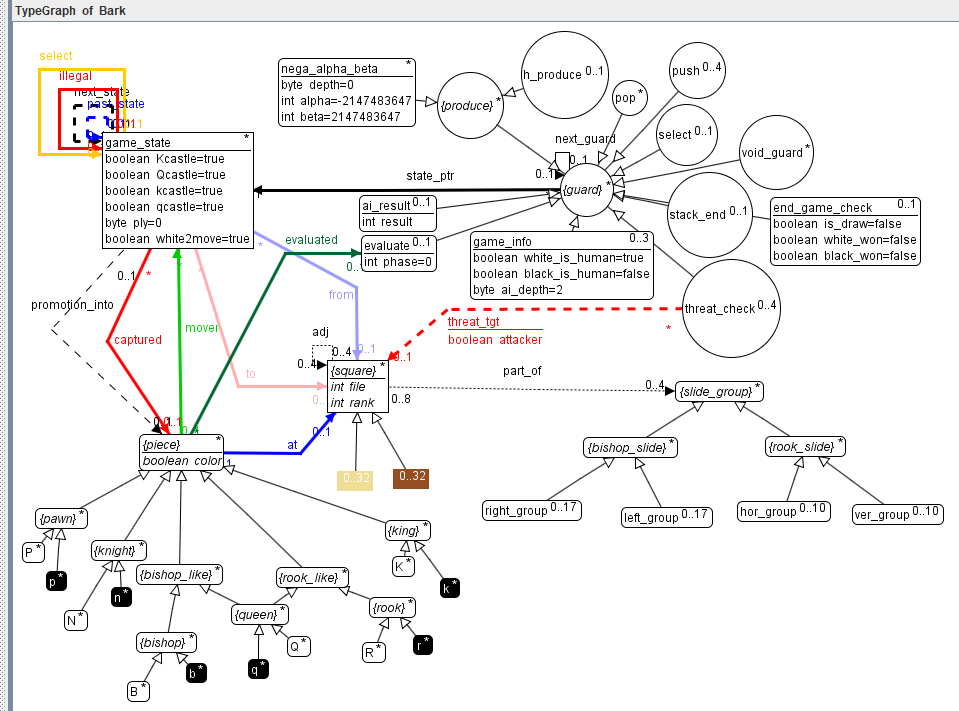
\includegraphics[width=.8\linewidth]{images/type_graph.png}
        \caption{The type graph of the system.}
    \end{figure}

    \paragraph{Construction by rules} We could have set up the board by hand (as we actually do to position the pieces and starting the game), but that would have been quite tedious because of the multiple edges needed to make it complete. Instead, we use a set of rules to produce it, which are as follows:
    \begin{enumerate}
        \item \texttt{produce\_first\_square} creates a first square of the board (the white top left square, \texttt{file=0} and \texttt{rank=7}), if it has not been created yet. This is then used as a seed for the rest of the construction.
        \begin{figure}[H]
            \centering
            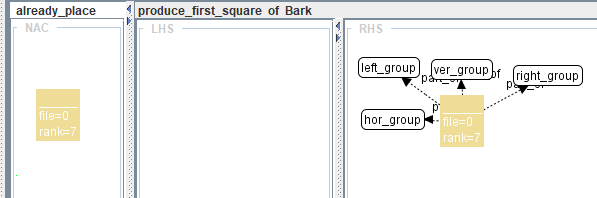
\includegraphics[width=.8\linewidth]{images/produce_first_square.png}
            \caption{\texttt{produce\_first\_square}}
        \end{figure}

        \item \texttt{produce\_top\_rank\_b/w} respectively create black and white squares of the top rank, if the they have not been created yet.
        \begin{figure}[H]
            \centering
            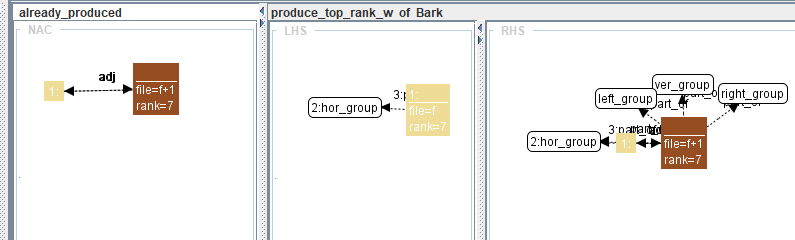
\includegraphics[width=.8\linewidth]{images/produce_top_rank.png}
            \caption{\texttt{produce\_top\_rank}}
        \end{figure}

        \item \texttt{produce\_first\_file\_b/w} respectively create the black and white squares of the first file, if they have not been created yet.
        \begin{figure}[H]
            \centering
            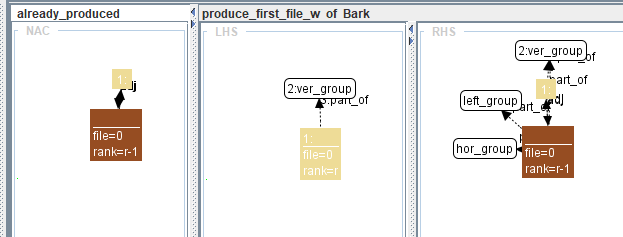
\includegraphics[width=.8\linewidth]{images/produce_first_file.png}
            \caption{\texttt{produce\_first\_file}}
        \end{figure}
    \end{enumerate}
    These first rules create the top rank and the left file of the board. The rest of the board is then created by applying:
    \begin{enumerate}
        \setcounter{enumi}{3}
        \item \texttt{produce\_square\_b/w} creates a black or white square, if it has not been created yet.
        \begin{figure}[H]
            \centering
            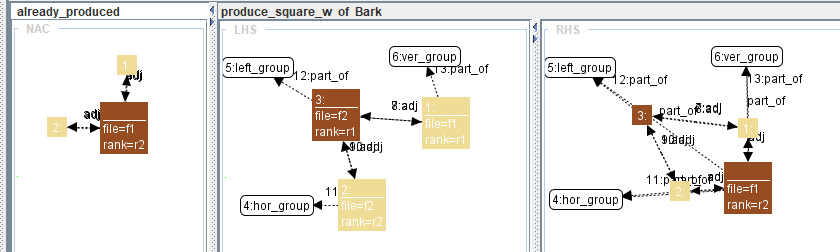
\includegraphics[width=.8\linewidth]{images/produce_square.png}
            \caption{\texttt{produce\_square}}
        \end{figure}

        \item \texttt{add\_right\_group} adds a \noderepr{right\_group} to squares on the last file, if it has not been added yet.
        \begin{figure}[H]
            \centering
            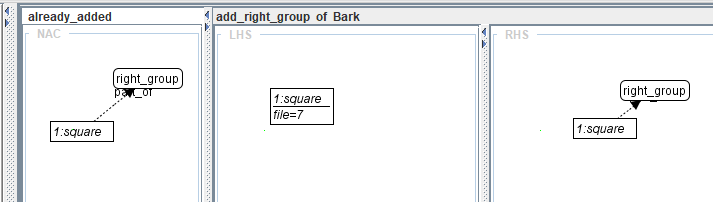
\includegraphics[width=.8\linewidth]{images/add_right_group.png}
            \caption{\texttt{add\_right\_group}}
        \end{figure}

        \item \texttt{produce\_right\_group} connects top-right to bottom-left the squares to the same group, if it has not been done yet.
        \begin{figure}[H]
            \centering
            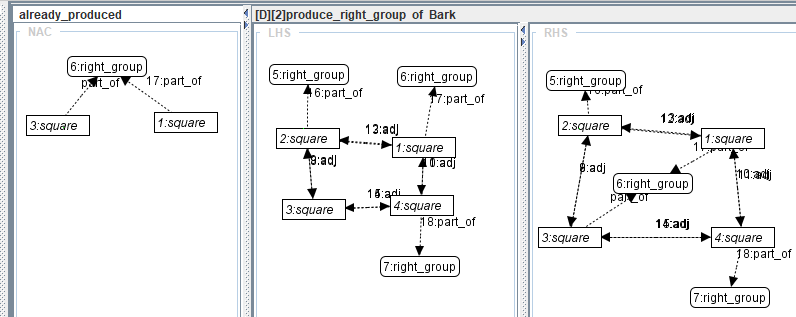
\includegraphics[width=.8\linewidth]{images/produce_right_group.png}
            \caption{\texttt{produce\_right\_group}}
        \end{figure}
    \end{enumerate}
    These rules are then applied in a loop until the board is complete.
    Of course, this is just a \emph{topological} description of the board, and, indeed, applying these rules doesn't result in a good-looking graph.
    \begin{figure}[H]
        \centering
        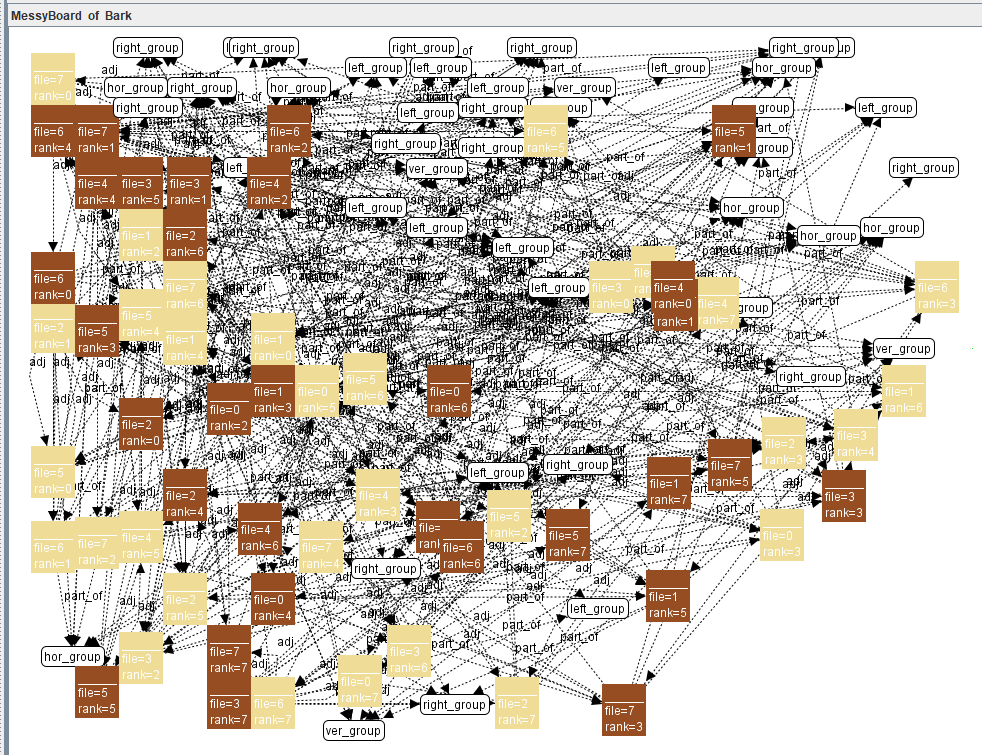
\includegraphics[width=.5\linewidth]{images/messy_board.png}
        \caption{The board after applying the rules.}
    \end{figure}
    To make it comprehensible, we order it by hand.
    \begin{figure}[H]
        \centering
        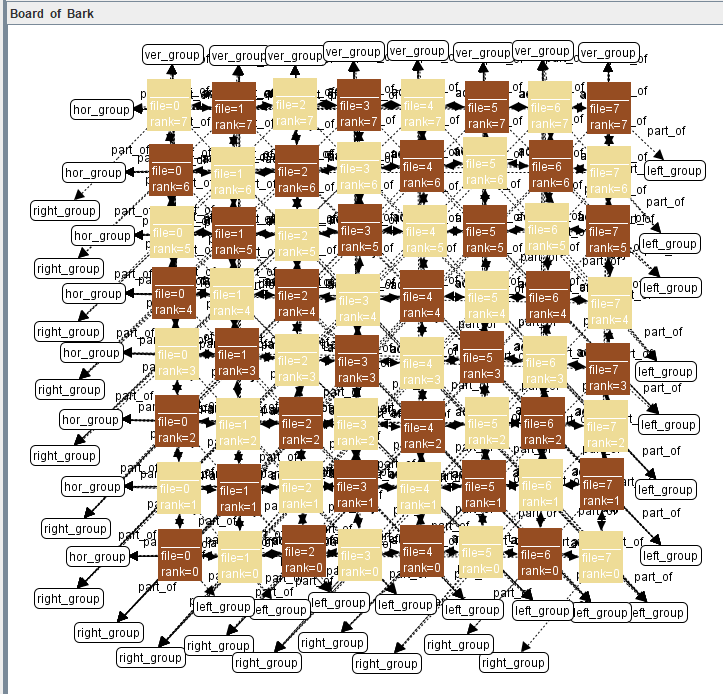
\includegraphics[width=.8\linewidth]{images/board.png}
        \caption{The board after hand-made ordering.}
    \end{figure}

    \section{Representing game states and enabling complex behaviors}
    Pieces are represented as nodes connected (via an \at) to the squares they are on. With a boolean \texttt{color} attribute (\texttt{false} for black pieces and \texttt{true} for white ones), \piece\ is the parent class, which is inherited by the \pawn, \knight, \bishoplike, \rooklike, and \king\ nodes. Specifically, the \bishoplike\ and \rooklike\ nodes are further inherited by \bishop, \rook, and \queen\ nodes, the latter of which is the only example of multiple inheritance in the system (as it moves like a rook and a bishop).
    A game state is not only composed by the pieces' positions on the board, but also by the information about the current rights to move, the castling rights, the last move, and the move counter (ply). This information is stored, explicitly via attributes and implicitly via edges, in the \gamestate.

    \paragraph*{Not only structure} Until now, we've only focused on defining a representation for the game, without including a description for its behavior. Graph rewriting mechanisms by themselves are enough to define a description for the rules of a game such as chess. But, to simplify the design of complex algorithms, we define another set of nodes all inheriting from \guard. These compose a stack (through the use of \nextguard) of operations which are used to enable only a subset of the rules at a time. Thanks to these, we were able to define the generation of moves, the evaluation of the board, the exploration of the game tree, and more.
    \begin{figure}[H]
        \centering
        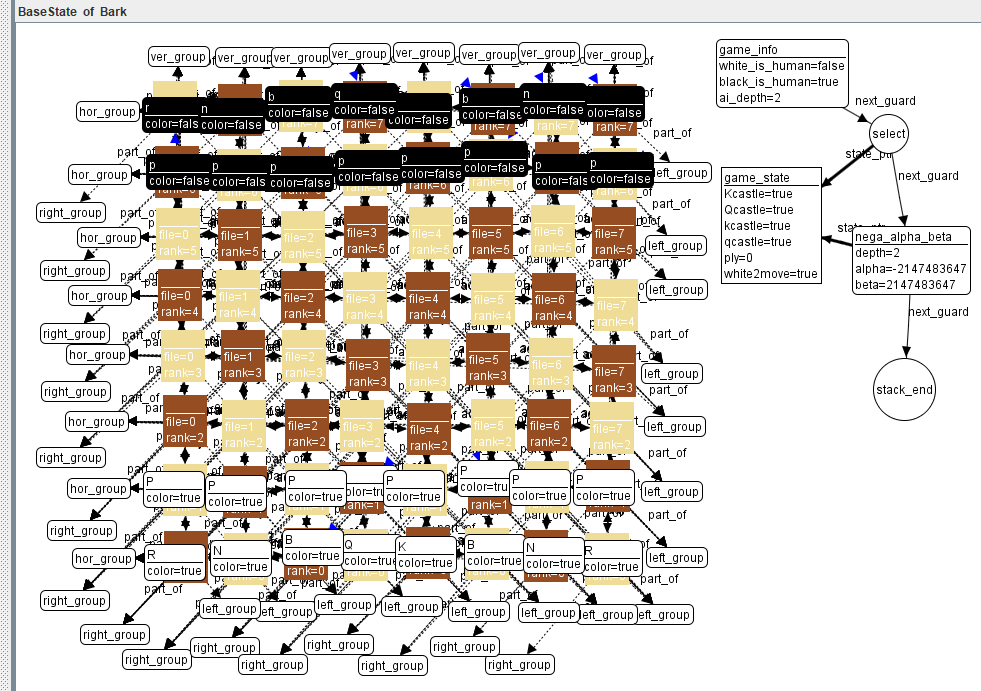
\includegraphics[width=.8\linewidth]{images/base_state.png}
        \caption{The starting configuration of the board.}
    \end{figure}
    Out of these \guard\ nodes, there are three that are designed for the control of the stack itself:
    \begin{enumerate}
        \item \gameinfo\ acts both as the start of the stack and as a container for the game information (which player is human and the depth of the search).
        \item \void\ has a usage akin to a "no-op" operation, as it is used to block all rules until it is removed.
        \item \stackend\ is the end of the stack, and it is used to signal which guard is at the top of the stack.
    \end{enumerate}
    All guards can have a \stateptr\ which connects them to a \gamestate.

    \section{Generating moves}
    \paragraph*{How it is done} As cited previously, in a traditional chess engine a lot of computations are done via "magic bitboards". These are perfect hashing algorithms which can trivialize a lot of checks, even the generation of movements. Without getting into the details, the moves are produced in a two-phase manner:
    \begin{enumerate}
        \item The result of every possible move is generated (via magic bitboards), without any forward checking (e.g. leaving the king in check), as that is usually too complex and slow to implement. The resulting set is called "pseudo-legal moves".
        \item For every possible resulting board, the king is checked for being in check. If it is, the move is discarded. This filtered set is called "legal moves".
    \end{enumerate}
    A further information to keep into account is that a chess engine usually enables "push" and "pop" operation on moves (i.e. to make a move and then undo it). This is done by keeping a stack of the boards, and pushing a new configuration every time a move is made. This is a very efficient way to implement the "undo" functionality, as it doesn't require to recompute the whole board every time. Furthermore, it is also used to implement the exploration of the game tree, as it allows backtracking to the previous state of the game.
    \paragraph*{How Bark does it} Bark, of course, cannot use magic bitboards. To produce a move, we have the \produce\ guard, which is "checked" upon by all the \texttt{move\_*} and \texttt{capture\_*} rules.
    Our method to generate moves is akin to the traditional one, but since we can afford to hold only a single board instance, it is more complex (and slow). We represent the game tree by connecting the \gamestate\ nodes: when pushing and popping the moves, instead of retrieving a stored configuration, we use the information present on the \gamestate\ to execute or revert the move by operating on the board instance.
    To implement push, pop and threat check operations we design multiple rules and their respective guards (\push, \pop, and \threatcheck), which we'll describe in further sections.

    To avoid repetitions, we first describe the patterns common to most (if not all) the \texttt{move\_*} and \texttt{capture\_*} rules:
    \begin{itemize}
        \item All rules produce a new \gamestate\ node, which is connected to the current one via a \nextstate\ edge. The moved piece gets a \mover\ connecting it to the new state, and the new state gets connected to the arriving square through a \tosquare\ edge. All but a couple rules append \pop, \threatcheck, and \push\ (which we define in the next section) to the stack.
        For the sake of the \threatcheck, moves will require the king of the moving color, to pass its position to \threatcheck.
        \item All rules have a NAC \texttt{already\_added} to ensure that the rule has not been applied yet.
        \begin{figure}[H]
            \centering
            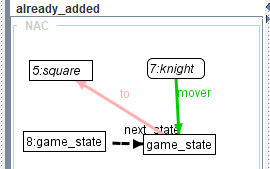
\includegraphics[width=.5\linewidth]{images/already_added_move.png}
            \caption{The \texttt{already\_added} NAC of the \texttt{move\_knight} rule.}
        \end{figure}
    \end{itemize}
    The rules are:
    \begin{enumerate}
        \item \texttt{move\_pawn} applies only when the next square is empty (\texttt{no\_blocker} NAC) and the pawn is moving forward (\texttt{r2==r1+(c?1:-1)}). It also checks that the move will not lead to a promotion (\texttt{r1!=(c?6:1)}), as it is handled by another rule.
        \begin{figure}[H]
            \centering
            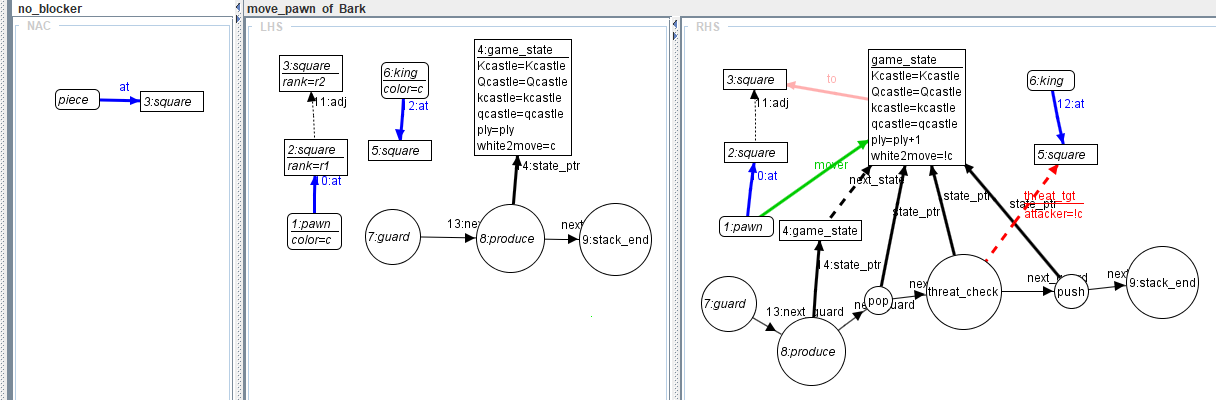
\includegraphics[width=.8\linewidth]{images/move_pawn.png}
            \caption{\texttt{move\_pawn}}
        \end{figure}
        \item \texttt{move\_pawn\_promotion\_white/black} apply like the \texttt{move\_pawn} rule, but only when the move leads to a promotion (i.e. the rank reached is either 7 or 0, based on moving color). These are among the only rules that don't append \pop, \threatcheck, and \push\ to the stack, but make a more complex update to it (as each possible promotion is a different move).
        \begin{figure}[H]
            \centering
            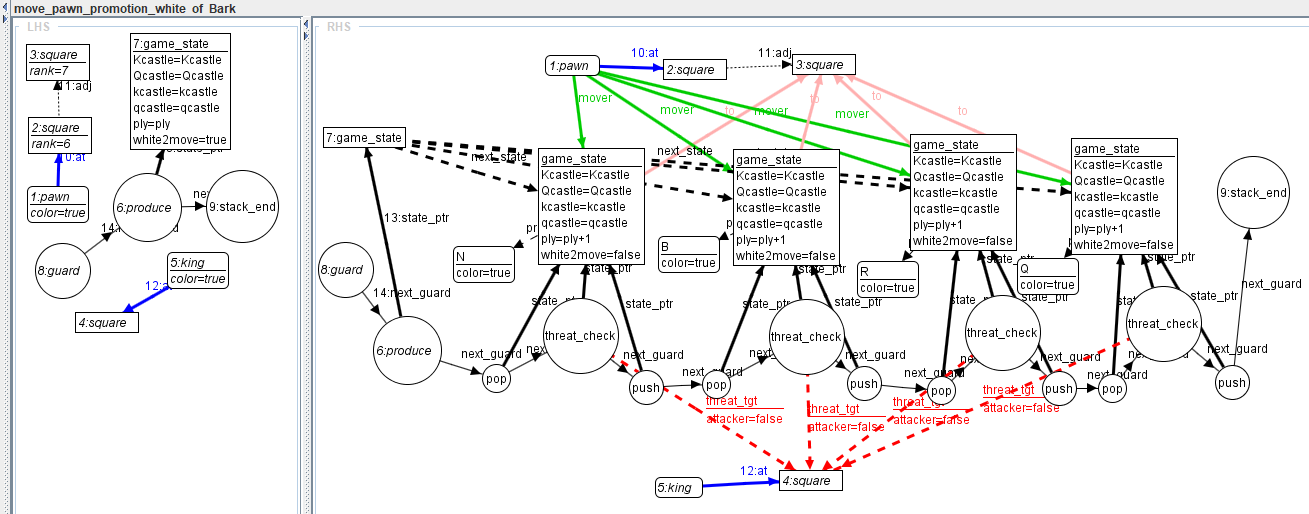
\includegraphics[width=.8\linewidth]{images/move_pawn_promotion_white.png}
            \caption{\texttt{move\_pawn\_promotion\_white}}
        \end{figure}
        \item \texttt{move\_pawn\_double} applies only when both next squares are empty (\texttt{no\_blocker} and \texttt{no\_middle\_blocker} NAC) and the pawn is moving forward (\texttt{r2==r1+(c?2:-2)}). It also checks that this is done only when it is the first move of the piece (\texttt{r1==(c?1:6)}).
        \begin{figure}[H]
            \centering
            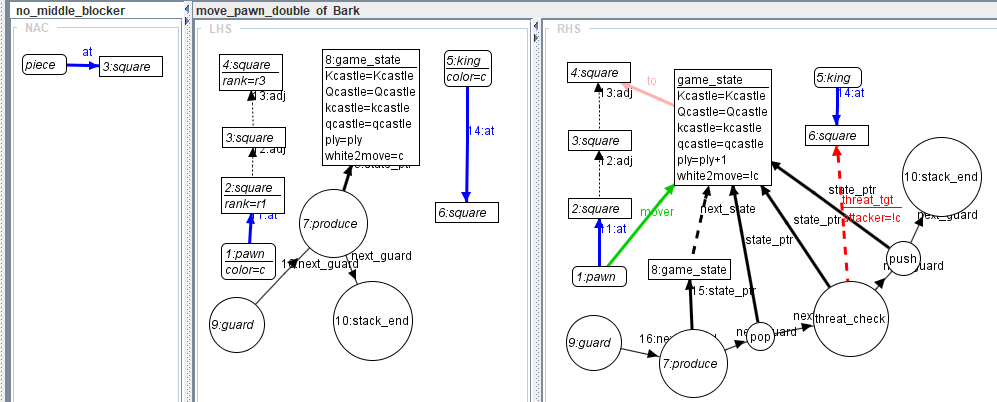
\includegraphics[width=.8\linewidth]{images/move_pawn_double.png}
            \caption{\texttt{move\_pawn\_double}}
        \end{figure}
        \item \texttt{capture\_pawn} applies only when the next square contains a foe or an en passant is possible (\texttt{normal\_capture | en\_passant} GAC) and the pawn is moving forward (\texttt{r2==r1+(c?1:-1)}). It also checks that the move will not lead to a promotion (\texttt{r1!=(c?6:1)}), as it is handled by another rule.
        \begin{figure}[H]
            \centering
            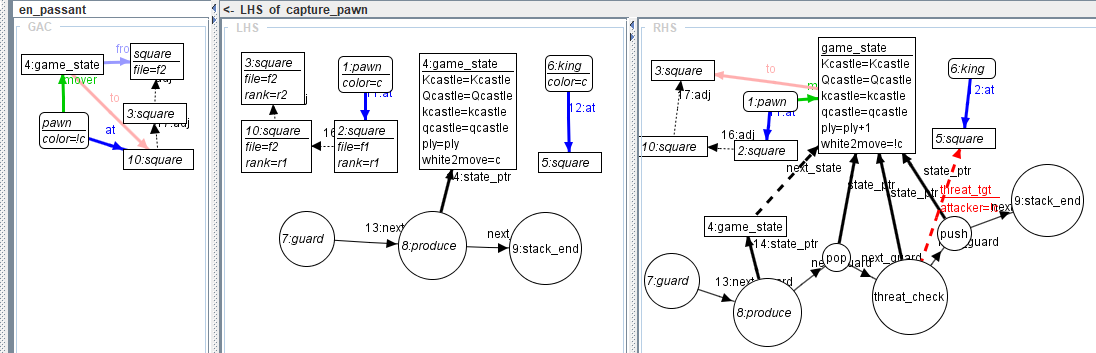
\includegraphics[width=.8\linewidth]{images/capture_pawn.png}
            \caption{\texttt{capture\_pawn}}
        \end{figure}
        \item \texttt{capture\_pawn\_promotion\_white/black} apply like the \texttt{capture\_pawn} rule, but only when the move leads to a promotion (i.e. the rank reached is either 7 or 0, based on moving color). Again, these are among the only rules that make a more complex update to the stack (as each possible promotion is a different move). Unlike the normal \texttt{capture\_pawn} rule, there is no need to check for en passant, as it is impossible when a promotion is happening.
        \begin{figure}[H]
            \centering
            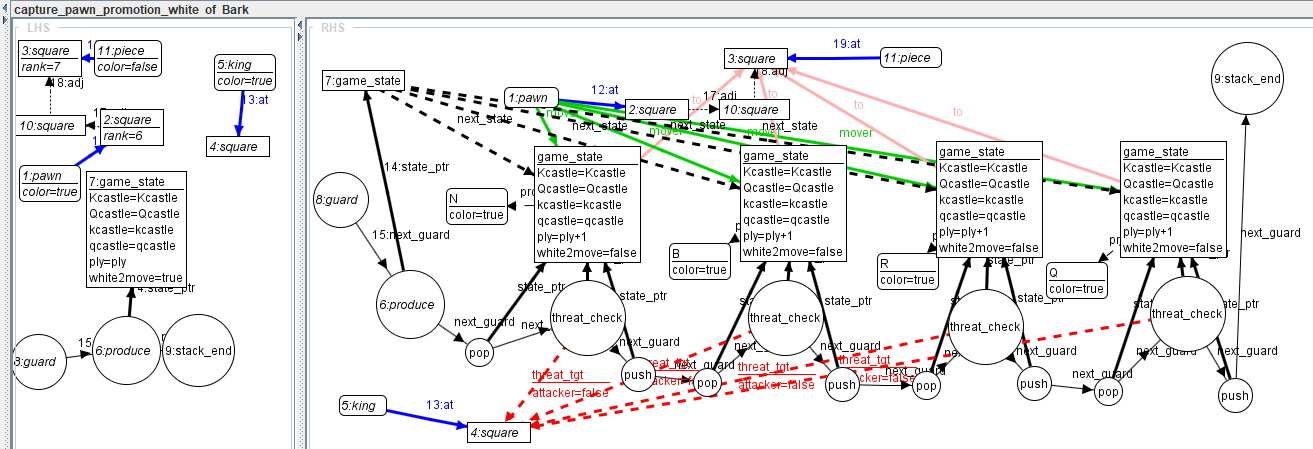
\includegraphics[width=.8\linewidth]{images/capture_pawn_promotion_white.png}
            \caption{\texttt{capture\_pawn\_promotion\_white}}
        \end{figure}
        \item \texttt{move\_knight} applies both to normal moves and captures (indeed, there doesn't exist a \texttt{capture\_knight}). To ensure that the piece can only move to an empty square or over a foe, a \texttt{no\_blocker} NAC is added.
        \begin{figure}[H]
            \centering
            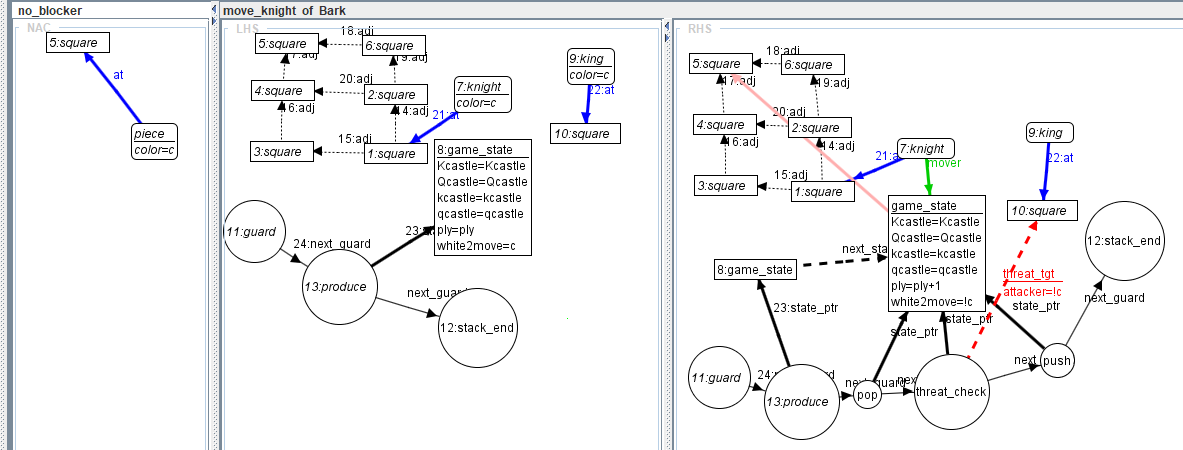
\includegraphics[width=.8\linewidth]{images/move_knight.png}
            \caption{\texttt{move\_knight}}
        \end{figure}
        \item \texttt{move\_bishop\_like} applies both to normal moves and captures, to both bishops and queens. To ensure that the piece can only move to an empty square or over a foe, a \texttt{no\_blocker} NAC is added. Furthermore, to ensure that there is no piece in between the starting and arriving squares, a \texttt{no\_middle\_blocker} NAC is added; this is possible only when the piece is in the same \bishopgroupnode, and it abides
        \begin{equation}\label{eq:slidegroupcheck}
            (8(f_3-f_1)+r_3-r_1)(8(f_3-f_2)+r_3-r_2)<0
        \end{equation}
        which is the condition for the middle ($f_3, r_3$) square to be between the starting ($f_1, r_1$) and arriving ($f_2, r_2$) squares.
        \begin{figure}[H]
            \centering
            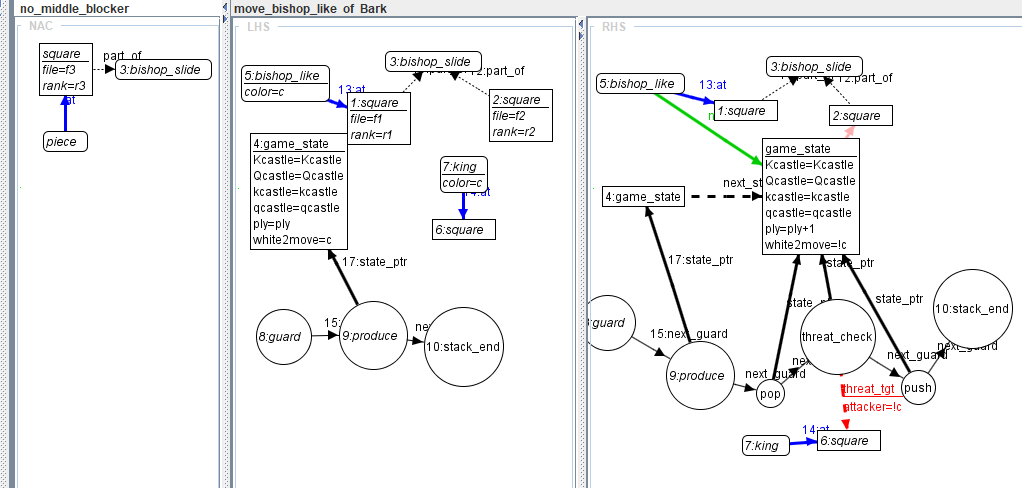
\includegraphics[width=.8\linewidth]{images/move_bishop_like.png}
            \caption{\texttt{move\_bishop\_like}}
        \end{figure}
        \item \texttt{move\_rook} applies both to normal moves and captures, but only to rooks (as these have to disable castling when it is the first time they move, queens do not). It works similarly to the \texttt{move\_bishop\_like} rule, with the only difference that the common slide group must be a \rookgroupnode. Again, the possible middle blocker at square ($f_3, r_3$) must abide \ref{eq:slidegroupcheck}.
        \begin{figure}[H]
            \centering
            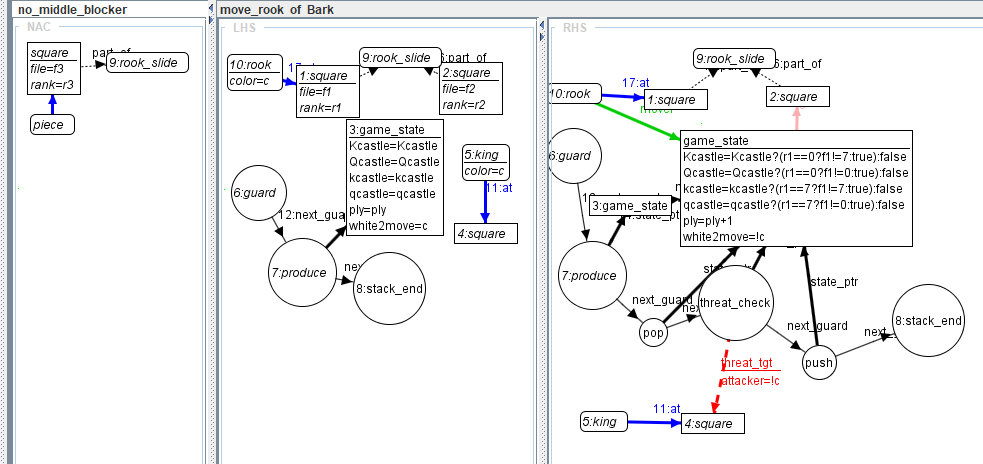
\includegraphics[width=.8\linewidth]{images/move_rook.png}
            \caption{\texttt{move\_rook}}
        \end{figure}
        \item \texttt{move\_queen} acts equivalently to \texttt{move\_rook}, with the only exception that it doesn't disable castling.
        \begin{figure}[H]
            \centering
            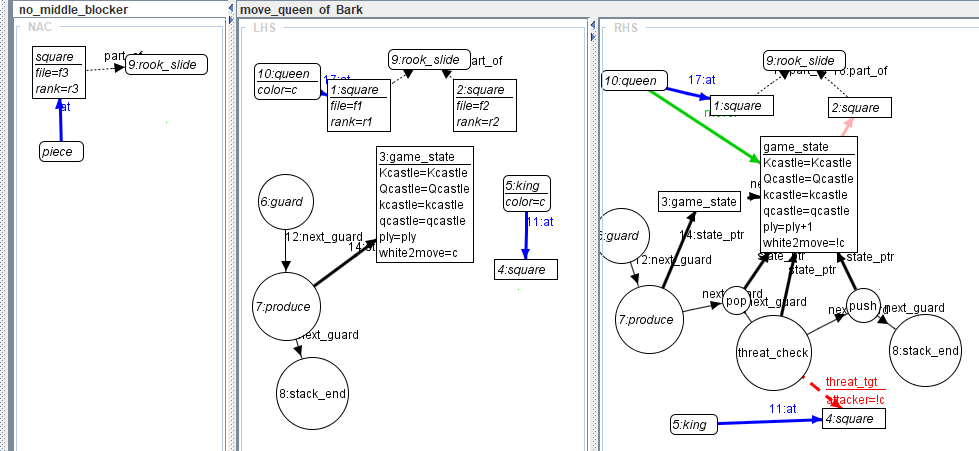
\includegraphics[width=.8\linewidth]{images/move_queen.png}
            \caption{\texttt{move\_queen}}
        \end{figure}
        \item \texttt{move\_king\_adj} applies both to normal moves and captures. To ensure that the piece can only move to an empty square or over a foe, a \texttt{no\_blocker} NAC is added. Of course, as it is the king itself that is moving, the \threatcheck\ checks on the arriving square, also, as the king is moving, the castling rights are updated.
        \begin{figure}[H]
            \centering
            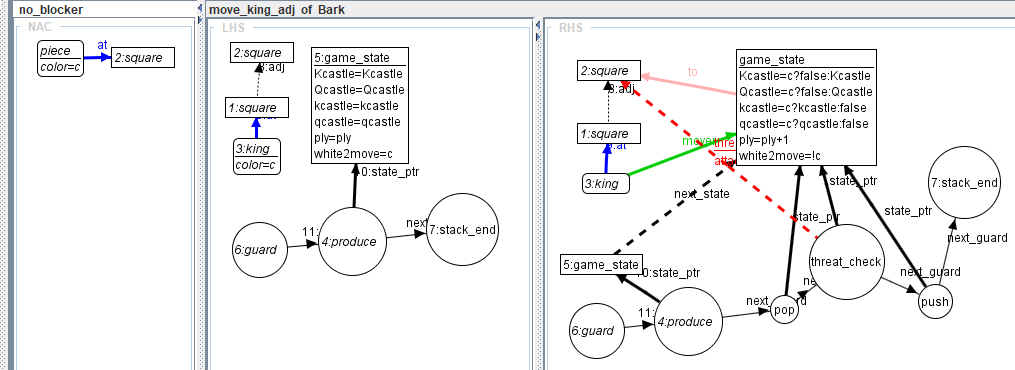
\includegraphics[width=.8\linewidth]{images/move_king_adj.png}
            \caption{\texttt{move\_king\_adj}}
        \end{figure}
        \item \texttt{move\_king\_diag} acts the same as \texttt{move\_king\_adj}, the only difference is in the diagonal moves.
        \begin{figure}[H]
            \centering
            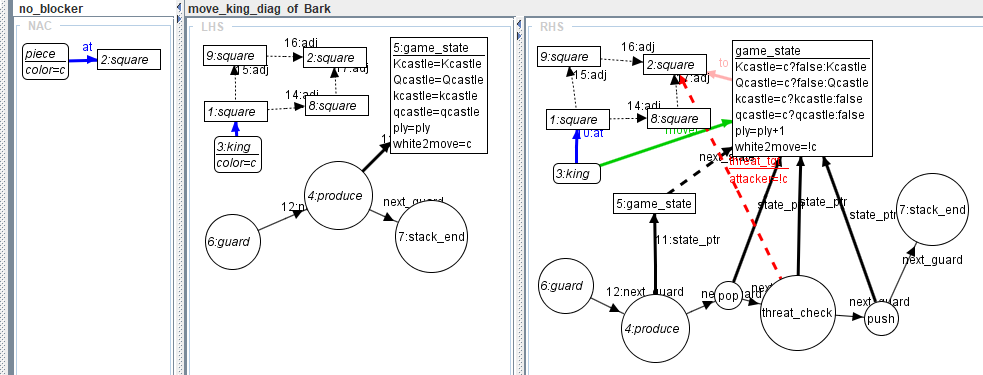
\includegraphics[width=.8\linewidth]{images/move_king_diag.png}
            \caption{\texttt{move\_king\_diag}}
        \end{figure}
        \item \texttt{move\_kingside/queenside\_castle} execute castling (if it is enabled in the current \gamestate, \texttt{c?Kcastle:kcastle} and \texttt{c?Qcastle:qcastle}). They also check that the squares between the king and the rook are empty (\texttt{no\_blocker*} NACs). As castling can only be done when the king is not in check (or moving across checked squares), these are the only moves that append \threatcheck\ to the stack before \push. Of course the resulting game state has the castling rights updated.
        \begin{figure}[H]
            \centering
            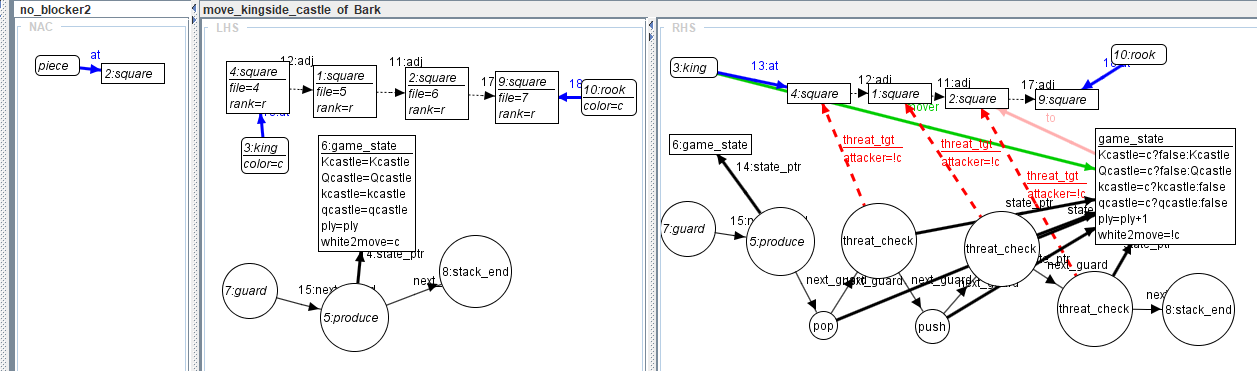
\includegraphics[width=.8\linewidth]{images/move_kingside_castle.png}
            \caption{\texttt{move\_kingside\_castle}}
        \end{figure}
    \end{enumerate}
    \section{Push, pop, and threat check}
\end{document}

